% LaTeX resume using res.cls
\documentclass[margin]{res}
\usepackage[english]{babel} % Should enable hyphenation
\usepackage{graphicx}
\usepackage{enumerate}
\usepackage{amsmath}
\usepackage{array}
\usepackage{hyperref}
%\usepackage{revnum}

%\usepackage{helvetica} % uses helvetica postscript font (download helvetica.sty)
%\usepackage{newcent}   % uses new century schoolbook postscript font 
\setlength{\resumewidth}{7.25in} % set width of text portion
\hyphenation{nano-fluidics}
\hyphenation{Micro-channels}
\hyphenation{refri-gera-tors}
\hyphenation{Local-ized}
\hyphenation{Electro-phoresis}
\hyphenation{AC-Dielectro-phoresis}
\hyphenation{Kon-vek-si-yon-la}
\hyphenation{micro-channel}
\hyphenation{mecha-nics}
\begin{document}

%\usepackage[T1]{fontenc}
%\usepackage[latin5]{inputenc}
\oddsidemargin -0.25in 

% \sl will be bold italic in New Century Schoolbook (or ny postscript font) and just slanted in Computer Modern (default) font

% Center the name over the entire width of resume:
\begin{tabular}{ p{4.25in} m{2in}}
{\LARGE\bf Kamil ÜNSAL}  &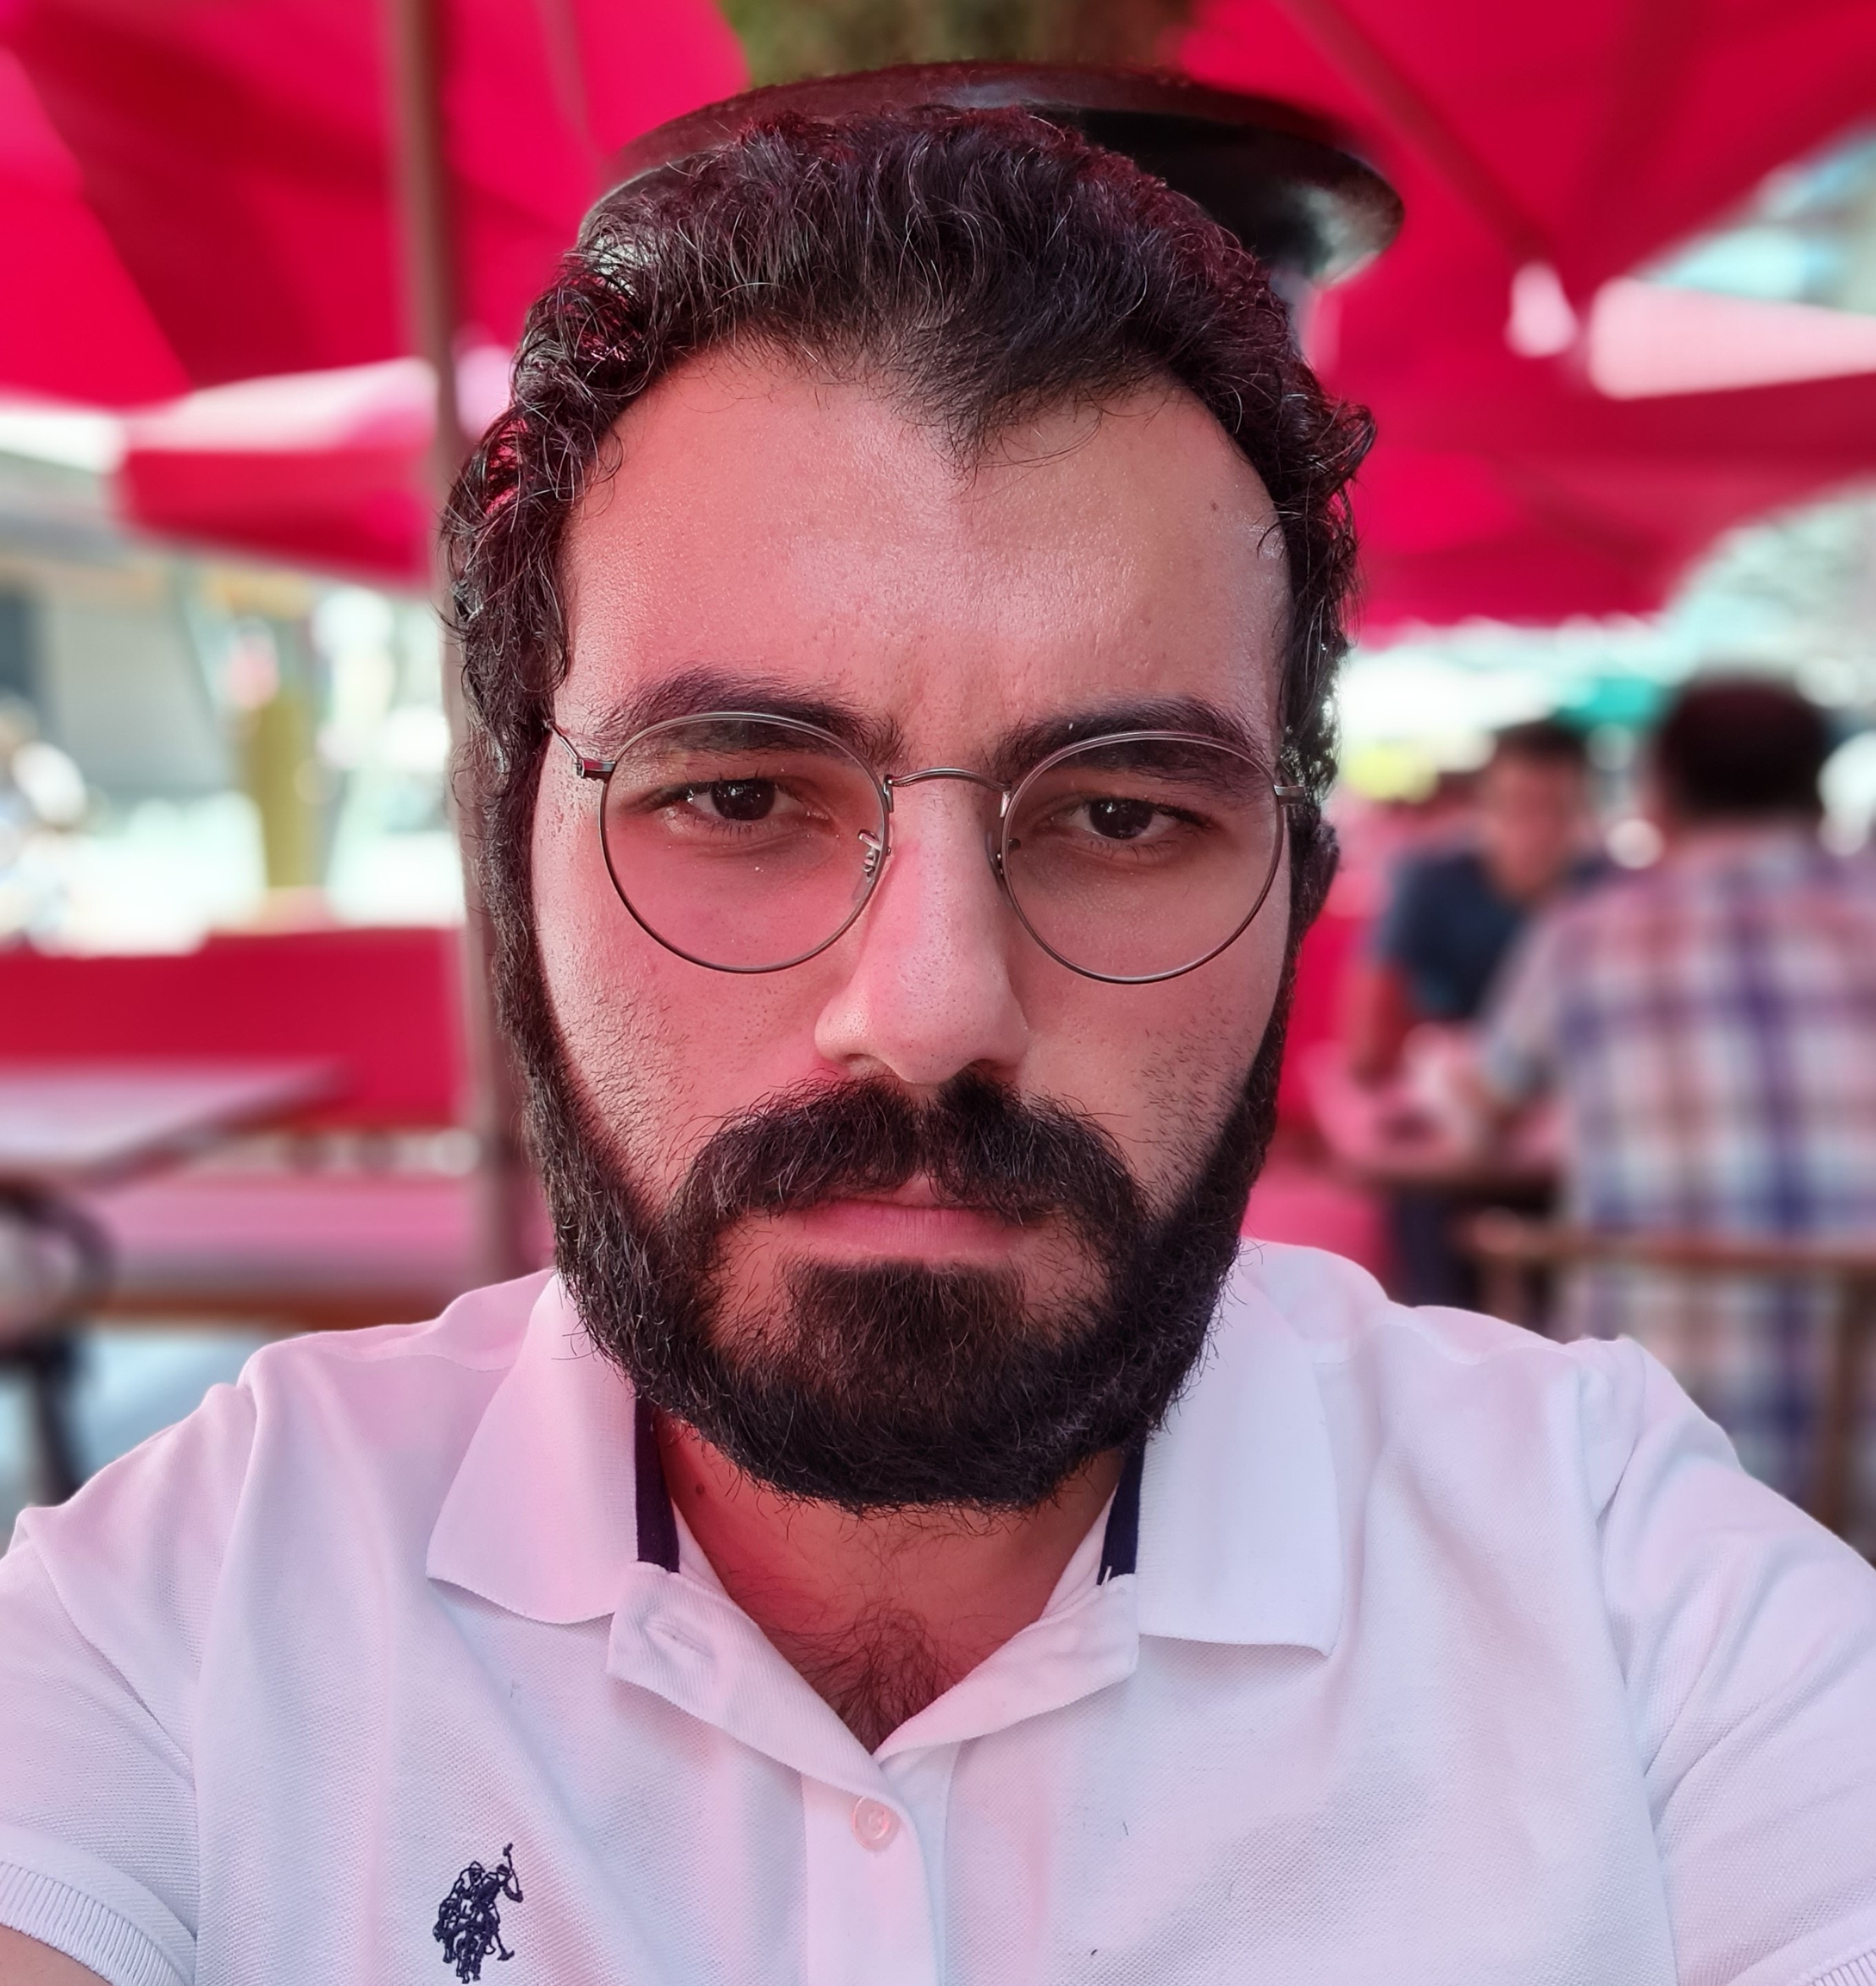
\includegraphics[height=1 in]{kmluns.jpg} \\

\end{tabular}
%\moveleft.5\hoffset\centerline{\LARGE\bf Barbaros \c{C}etin, Ph.D.}
 
% Draw a horizontal line the whole width of resume:
\moveleft\hoffset\vbox{\hrule width\resumewidth height 1pt}\smallskip
% address begins here
% Again, the address lines must be centered over entire width of resume:
% \moveleft.5\hoffset\centerline{Vanderbilt University, Department of Mechanical Engineering}

\begin{resume}

\section{\mysidestyle \textbf{CONTACT INFORMATION}}
\begin{tabular}{@{} l l l l}
Mobile & :  \href{tel:905064227868}{+90 506 422 7868}  &  Linkedin & :  \href{https://www.linkedin.com/in/kmluns?locale=en_US}{kmluns} \\
E-mail & :  \href{mailto:kmlunsl@gmail.com}{kmlunsl@gmail.com} & GitHub & :  \href{https://github.com/kmluns}{kmluns} \\
\end{tabular}


\section{\mysidestyle \textbf{CAREER PROFILE}}
\textbf{2019 - } Milsoft Software Technologies, Senior Software Engineer \\
\newline
\textbf{2018 –} ICterra Information and Communication Technologies, Software Engineer \\	
\newline
\textbf{2017 –} BEAM Tecnology, Common Criteria Evaluator Assistant \\	
\newline

\section{\mysidestyle \textbf{AREAS of INTEREST}} Web Technologies , Natural Language Processing, Deep Learning \\[0.08in]


\section{\mysidestyle \textbf{PERSONAL\\INFORMATION}}
\textbf{Nationality /Citizenship:} Turkish/Turkey\\
\textbf{Date/Place of birth:} 1994/Çankırı, Turkey\\
\textbf{Martial Status:} Single\\
\textbf{Driving License:} B (2012)\\
\textbf{Languages:} English(Intermediate)\\

\section{\mysidestyle \textbf{EDUCATION}}
\textbf{Hacettepe University,} Ankara, Turkey \\	
{\sl Bachelor of Science,} Computer Science (3.04/4.00)  \hfill {\bf 2012 - 2017} \\[0.08in] \newline
\textbf{Çankırı Süleyman Demirel Science High School}, Çankırı, Turkey \hfill {\bf 2008 - 2012} \\[0.08in]


\section{\mysidestyle \textbf{WORK\\EXPERIENCE}}
\textbf{Milsoft Software Technologies} (Full Time) \\ {\bf November 2019 –  Currently } \\
\begin{itemize}
    \item 
    \textbf{Tactical Data Link Product} \\
    \textit{Senior Software Engineer} \\
    \\
    The product provides the Data Link capability to share tactical information with other Link 16, Link 22, Link 11 capable platforms. The product is capable of forwarding data link messages among different link systems using either Link 11/16/22. I am developing the Link 16 Messages.  \\
    \begin{tabular}{@{} l l}
        \textbf{Technologies} & :   Java, C++, DDS, Maven \\ 
        \textbf{Processes and tools} & :  IntelliJ, Visual Studio, JIRA, Confluence, FishEye \\
    \end{tabular}
    \\
    Ankara, Turkey \hfill {\bf November 2019 – December 2020 }\\[0.08in] \newline
\end{itemize}
\textbf{ICterra Information and Communication Technologies} (Full Time) \\ {\bf May 2018 – November 2019 } \\
\begin{itemize}
    \item 
    \textbf {Cancer Patients Follow Up App} \\
    \textit{Full Stack Developer} \\
    \\
    The project is a follow up app for cancer patients. The project includes types of cancer, the status of patients, substances used in drugs. I developed patient monitoring web application using Spring Boot and ReactJS   \\
    \begin{tabular}{@{} l l}
        \textbf{Technologies} & :   Java, JavaScript, Spring Boot, ReactJS, MYSQL, JPA \\ 
        \textbf{Processes and tools} & :  IntelliJ, Visual Studio Code, JIRA, Confluence, FishEye + Crucible \\
    \end{tabular}
    \\
    Ankara, Turkey
    \hfill {\bf Jun 2019 – November 2019 }\\[0.08in] \newline
\end{itemize}
% \begin{itemize}
%     \item 
%     \textbf {AED(Automated External Defibrillator) Service Software} \\
%     \textit{Software Engineer} \\
%     \\
%     The project is an embedded application that configure the AED device over a serial channel. I developed the service software that retrieves the data contained in the AED device, examining and recording this data. I coded observer, MVC, thread safe singleton design patterns for this application.   \\
%     \begin{tabular}{@{} l l}
%         \textbf{Technologies} & :  QT, C++, MYSQL \\ 
%         \textbf{Processes and tools} & :  JIRA, Confluence, FishEye + Crucible \\
%     \end{tabular}
%     \\
%     Ankara, Turkey
%     \hfill {\bf July 2019 – October 2019 }\\[0.08in] \newline
% \end{itemize}
\begin{itemize}
    \item 
    \textbf {Mobile XRAY Device} \\
    \textit{Software Engineer} \\
    \\ 
    The device that has an x-ray tube can shoot x-rays and move. I developed the application written in Java. I coded using multi-thread, RMI, JNI technologies with Java programming language.    \\
    \begin{tabular}{@{} l l}
        \textbf{Technologies} & : Java, MYSQL, C++, JNI, RMI, Spring Framework \\ 
        \textbf{Processes and tools} & :  Eclipse, JIRA, Confluence, FishEye + Crucible \\
    \end{tabular}
    \\
    Ankara, Turkey
    \hfill {\bf May 2019 – November 2019 }\\[0.08in] \newline
\end{itemize}
\textbf{BEAM Technology} (Full Time) \\ {\bf November 2017 – May 2018 }\\
\begin{itemize}
    \item 
    \textbf {SOC(Security Operation Center) Project} \\
    \textit{Software Engineer} \\
    \\
    I created the architecture of the soc. I've set the settings for installing the applications. I made them work in an integrated way.    \\
    \begin{tabular}{@{} l l}
        \textbf{Technologies} & :   Elasticsearch, Logstash, Kibana, Snort, Security Onion, Docker \\ 
        \textbf{Processes and tools} & :  Slack \\
    \end{tabular}
    \\
    Ankara, Turkey
    \hfill {\bf April 2018 – May 2018 }\\[0.08in] \newline
\end{itemize}
\begin{itemize}
    \item 
    \textbf {Olta.la Project} \\
    \textit{Full Stack Developer} \\
    \\
    The project is that the users can send phishing e-mails. Also, users can create training for creating security awareness. I developed project using Spring Boot and AngularJS technologies.   \\
    \begin{tabular}{@{} l l}
        \textbf{Technologies} & :  Java, MongoDB, Spring MVC, AngularJS \\ 
        \textbf{Processes and tools} & :  IntelliJ \\
    \end{tabular}
    \\
    Ankara, Turkey
    \hfill {\bf Jan 2018 – May 2018 }\\[0.08in] \newline
\end{itemize}
\begin{itemize}
    \item 
    \textbf {Report Follow Up Project} \\
    \textit{Full Stack Developer} \\
    \\
    The project is that all managers can manage reports belong to employers in an organization. I worked as full stack developer in this project.    \\
    \begin{tabular}{@{} l l}
        \textbf{Technologies} & :  Java, MongoDB, Spring MVC, Angular5 \\ 
        \textbf{Processes and tools} & :  IntelliJ \\
    \end{tabular}
    \\
    Ankara, Turkey
    \hfill {\bf March 2018 – April 2018 }\\[0.08in] \newline
\end{itemize}
\begin{itemize}
    \item 
    \textbf {Source Code Security Analysis} \\
    \textit{Common Criteria Evaluator Assistant} \\
    \\
    I analyzed for security vulnerabilities in source code for "Common Criteria Certification" process.   \\
    \begin{tabular}{@{} l l}
        \textbf{Technologies} & :  Java, .NET, NodeJS, PHP \\ 
        \textbf{Processes and tools} & :  Burp Suite, IntelliJ, CLion, PHPStorm, Visual Studio 2015 \\
    \end{tabular}
    \\
    Ankara, Turkey
    \hfill {\bf December 2017 – May 2018 }\\[0.08in] \newline
\end{itemize}
\section{\mysidestyle \textbf{TECHNICAL SKILLS, \\ TOOLS \& \\ METHODS}} 
{\sl \textbf{Qualifications :}}  Java, Spring Boot, React, Typescript \\[0.03in]
{\sl \textbf{Project Management Tools :}}  Trello, JIRA, Confluence  \\ [0.03in]
{\sl \textbf{Internet / Communication / Networks :}} Burp Suite, Wireshark, TCP/IP \\ [0.03in]
{\sl \textbf{Operating Systems :}}  Linux (Ubuntu, CentOS, Kali Linux, Fedora), Windows \\[0.03in]
{\sl \textbf{Development Tools :}}  IntelliJ, Eclipse, Spyder, Visual Studio, VSCode  \\ [0.03in]
{\sl \textbf{Programming Languages :}} Java, TypeScript, JavaScript, Python, C/C++, C\# \\ [0.03in]
{\sl \textbf{Web Technologies :}} Spring Boot, ReactJS, React-Native, Angular, Ionic \\ [0.03in]
{\sl \textbf{Databases :}}  MongoDB, MYSQL, Elasticsearch \\[0.03in]


\section{\mysidestyle \textbf{TRAINING \\ AND \\ CERTIFICATES}} 
ICterra React Hackathon TEAM 2018 – 10.08.2018 \\
Deep Learning Workshop – NVIDIA DLI - 20.10.2017 \\
Sony Cyber Security Workshop – 28.04.2017 \\
AB2016 Siber Saldırı ve Savunma Atölyesi - 2016 \\
AB2015 Kriptoloji-2 – 2015 

\end{resume}
\end{document}




